% Author: Till Tantau
% Source: The PGF/TikZ manual
\documentclass{article}

\usepackage{tikz}
\usepackage{verbatim}

\begin{document}
\pagestyle{empty}

\begin{comment}
:Title: Automata
:Tags: Manual, Automata, Foreach, Graphs

This example is from the System layer  title page of the TikZ and PGF manual.

| Author: Till Tantau
| Source: The PGF/TikZ manual

\end{comment}
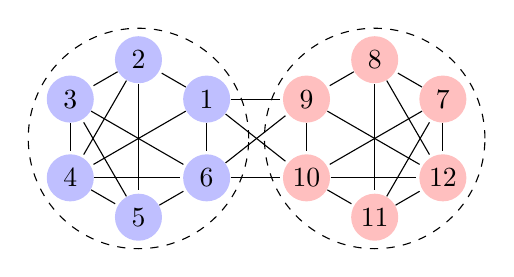
\begin{tikzpicture}[shorten >=1pt,-]
  \tikzstyle{vertex}=[circle,fill=black!25,minimum size=17pt,inner sep=0pt]

  \foreach \name/\angle/\text in {P-1/30/1, P-2/90/2, P-3/150/3, P-4/210/4, P-5/270/5, P-6/330/6}
    \node[vertex,xshift=6cm,yshift=.5cm,fill=blue!25] (\name) at (\angle:1cm) {$\text$};

  \foreach \name/\angle/\text in {Q-1/30/7, Q-2/90/8, Q-3/150/9, Q-4/210/10, Q-5/270/11, Q-6/330/12}
    \node[vertex,xshift=9cm,yshift=.5cm,fill=red!25] (\name) at (\angle:1cm) {$\text$};

    \foreach \from/\to in {1/2,2/3,3/4,3/6,4/5,5/3,1/4,2/5,2/4,4/6,5/6,1/6}
    { \draw (P-\from) -- (P-\to);}
    \foreach \from/\to in {1/2,2/3,3/4,4/5,5/1,1/4,2/5,3/6,2/6,4/6,5/6,1/6}
    {\draw (Q-\from) -- (Q-\to); }

  \foreach \from/\to in {1/3,1/4,6/3,6/4}
    { \draw (P-\from) -- (Q-\to); }
    
%    برای رسم دایره‌ها
 \draw[dashed] (6,.5) ellipse (1.4cm and 1.4cm);
 \draw[dashed] (9,.5) ellipse (1.4cm and 1.4cm);

%رسم بیضی‌ها و رنگ کردن مجدد نودهای میانی
%   \foreach \name/\angle/\text in {P-1/30/1, P-6/330/6}
%       \node[vertex,xshift=6cm,yshift=.5cm,fill=blue!55!red!25] (\name) at (\angle:1cm) {$\text$};
%  \foreach \name/\angle/\text in { Q-3/150/9, Q-4/210/10}
%    \node[vertex,xshift=9cm,yshift=.5cm,fill=blue!25!red!25] (\name) at (\angle:1cm) {$\text$};

% \draw[dashed] (6.6,.5) ellipse (2.1cm and 1.4cm);
% \draw[dashed] (8.4,.5) ellipse (2.1cm and 1.4cm);

\end{tikzpicture}

\end{document}